\documentclass[a4paper,11pt, twoside]{report}
\usepackage{hyperref}
\usepackage{graphicx}
\usepackage[backend=biber, sorting=none, style=ieee]{biblatex}
\addbibresource{library.bib}

\begin{document}

\section*{Relazione progetto basi di dati}
\subsection*{Michele Ceccacci, mat. 0001027124}
\subsubsection*{\today}

\subsection*{Introduzione}
L' obiettivo di questa relazione è parallelizzare il programma circles.c usando openMP e MPI. 
Questo programma calcola prende cerchi sovrapposti e li sposta minimizzando le loro sovrapposizioni.
Ho usato la funzionalità movie per verificare la correttezza di entrambe le implementazioni in maniera visuale. 
Inoltre ho cercato di vedere se il codice esempio (non parallelizzato) avesse un numero di overlap simili a ogni iterazione. Ho cercato di sfruttare la versione di MPI (che non ha race condition, dato che ogni processo ha le sue variabili) 
per cercare race condition nella versione OMP (dato che i thread condividono lo stesso address space di default). 
L' approccio usato per entrambi i programmi paralleli è stato quello di cercare di ottenere codice corretto,
e poi parallellizzarlo e guadagnare più performance possibile.
\subsection*{Versione OpenMP}
Parallelizzato usando \textbf{openMP} \cite{openMP}.
Ho deciso di estrarre i delta x e y nella struttura circle in array separati, così da poterli usare insieme alla primitiva \textbf{OpenMP reduce} \cite{omp_reduce}, rendendo il codice piu chiaro.
Nella funzione reduce\_forces, ho parallellizzato solo il loop esterno, che non presenta nessuna loop-carried dependency.
Dato che il workload è molto sbilanciato e le performance non erano ottimali, ho poi deciso di usare dynamic scheduling.
Ho usato il costrutto openMP parallel for, e ho definito le variabili con default(none), in maniera da dover pensare al significato di ogni singola variabile e non lasciare ambiguità nel mio codice.
Ho definito variabili che non vengono modificate come shared per evitare copie inutili.
Inoltre ho sempre usato il costrutto reduce di openMP per computare le somme sia degli offset che della variabile che rappresenta il numero di sovrapposizioni.
Questo mi ha consentito di evitare race condition, e di rendere il mio codice più semplice senza impattare in alcun modo la performance.
Ho eseguito il problema su una size base di 2000 cerchi, e ho fatto 5 iterazioni separate per ogni combinazione di input, in modo da ridurre la possibilità di avere risultati imprecisi.
I tempi nelle tabelle sono misurati in secondi.
\begin{table}[!ht]
    \centering
    \begin{tabular}{|l|l|l|l|l|l|l|}
    \hline
        threads & t1 & t2 & t3 & t4 & t5 & ~ \\ \hline
        1 & 0.984081 & 0.984136 & 0.983351 & 0.980449 & 0.984029 & ~ \\ \hline
        2 & 0.507617 & 0.501525 & 0.495320 & 0.499768 & 0.503177 & ~ \\ \hline
        3 & 0.336122 & 0.334336 & 0.337910 & 0.335685 & 0.334806 & ~ \\ \hline
        4 & 0.254741 & 0.257792 & 0.254491 & 0.257680 & 0.253694 & ~ \\ \hline
        5 & 0.204755 & 0.204981 & 0.204034 & 0.201425 & 0.201518 & ~ \\ \hline
        6 & 0.173564 & 0.173434 & 0.173012 & 0.173855 & 0.174283 & ~ \\ \hline
        7 & 0.149820 & 0.148868 & 0.151582 & 0.150275 & 0.148041 & ~ \\ \hline
        8 & 0.134840 & 0.147915 & 0.143373 & 0.129060 & 0.133693 & ~ \\ \hline
        9 & 0.122246 & 0.122463 & 0.126822 & 0.132121 & 0.132055 & ~ \\ \hline
        10 & 0.118163 & 0.115866 & 0.113696 & 0.116546 & 0.119328 & ~ \\ \hline
        11 & 0.103750 & 0.102452 & 0.111288 & 0.112172 & 0.104592 & ~ \\ \hline
        12 & 0.107195 & 0.108961 & 0.101341 & 0.156694 & 0.206630 & ~ \\ \hline
    \end{tabular}
\end{table}
\newline
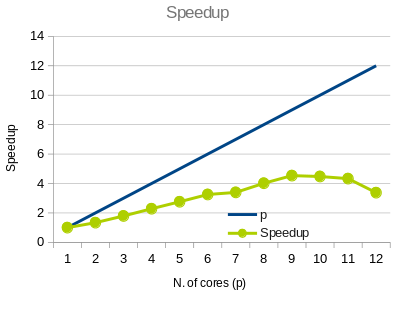
\includegraphics[scale=0.5]{images/omp_speedup.png}
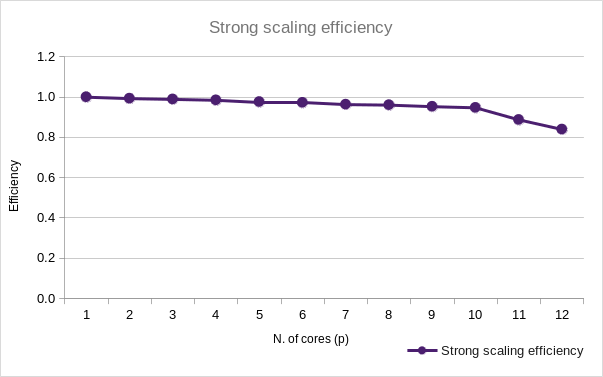
\includegraphics[scale=0.5]{images/omp_strong.png}
La ragione per cui lo speedup diminuisce nella dodicesima iterazione è che il thread probabilmente viene usato dal sistema operativo.
Dato che il carico è bilanciato dinamicamente, ogni thread prende una frazione del lavoro uguale agli altri, 
e le performance in weak scaling sono molto buone.
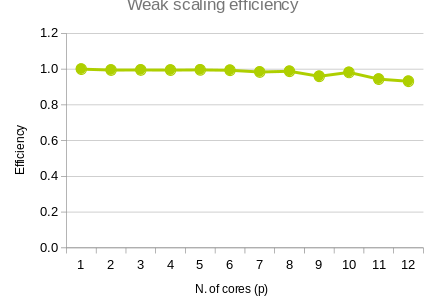
\includegraphics[scale=0.5]{images/omp_weak.png}
\begin{table}[!ht]
    \centering
    \begin{tabular}{|l|l|l|l|l|l|l|}
    \hline
        p & t1 & t2 & t3 & t4 & t5 & ~ \\ \hline
        1 & 0.497624 & 0.502653 & 0.497082 & 0.496878 & 0.498347 & ~ \\ \hline
        2 & 0.501651 & 0.495778 & 0.502095 & 0.499785 & 0.500418 & ~ \\ \hline
        3 & 0.499069 & 0.496452 & 0.496993 & 0.499587 & 0.496836 & ~ \\ \hline
        4 & 0.499963 & 0.495844 & 0.497311 & 0.498636 & 0.498090 & ~ \\ \hline
        5 & 0.503251 & 0.500397 & 0.501445 & 0.499359 & 0.500204 & ~ \\ \hline
        6 & 0.502926 & 0.499865 & 0.503116 & 0.502779 & 0.502013 & ~ \\ \hline
        7 & 0.502450 & 0.502578 & 0.501149 & 0.498879 & 0.501934 & ~ \\ \hline
        8 & 0.503764 & 0.503973 & 0.504111 & 0.500561 & 0.502809 & ~ \\ \hline
        9 & 0.510822 & 0.513545 & 0.502197 & 0.505757 & 0.506698 & ~ \\ \hline
        10 & 0.516669 & 0.507416 & 0.506557 & 0.507217 & 0.507029 & ~ \\ \hline
        11 & 0.521998 & 0.511696 & 0.526383 & 0.510572 & 0.506039 & ~ \\ \hline
        12 & 0.511261 & 0.608653 & 0.507164 & 0.516128 & 0.508778 & ~ \\ \hline
    \end{tabular}
\end{table}
\section*{Versione MPI}
Usando \textbf{MPI}\cite{mpi}, dato che ogni processo ha bisogno di ricevere un' array aggiornato con tutte le informazioni rilevanti ai cerchi, 
ho dovuto definire un nuovo data type circle, che ho potuto usare per inviare direttamente le informazioni. 
Questo mi consente di ridurre il numero di  \textbf{MPI\_Bcast} \cite{mpi_bcast} necessarie ad ogni iterazione. Dato che a ogni processo servono le
informazioni presenti in tutto l' array, e non solo una porzione, ho usato \textbf{MPI\_Bcast}\cite{mpi_bcast} per facilitare l' invio e non duplicare lavoro,
come sarebbe successo se avessi scelto di usare \textbf{MPI\_send} \cite{mpi_send} \textbf{MPI\_recv} \cite{mpi_recv}. 
Dopo aver calcolato i nuovi displacement sull'asse x e y, ho usato \textbf{MPI\_reduce} \cite{mpi_reduce} per agevolare le operazioni di somma.
In questo caso ho preferito codice piu semplice al definire una operazione di reduce custom,
che permette efficienza migliore rispetto all' usare direttamente primitive di livello più basso.
Ho eseguito il problema su una size base di 2000 cerchi, e ho fatto 5 iterazioni separate per ogni combinazione di input, in modo da ridurre la possibilità di avere risultati imprecisi.
I tempi sono misurati in secondi.
\newline
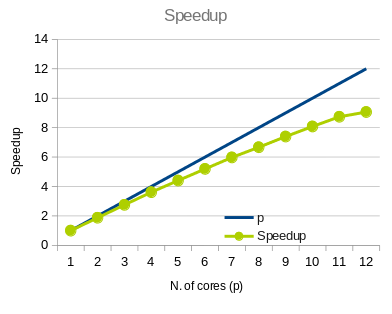
\includegraphics[scale=0.5]{images/mpi_speedup.png}
\begin{table}[!ht]
    \centering
    \begin{tabular}{|l|l|l|l|l|l|l|}
    \hline
        processi & t1 & t2 & t3 & t4 & t5 & ~ \\ \hline
        1 & 0.969648 & 0.971259 & 0.970024 & 0.971939 & 0.971256 & ~ \\ \hline
        2 & 0.729474 & 0.728466 & 0.731550 & 0.731297 & 0.729286 & ~ \\ \hline
        3 & 0.541049 & 0.542373 & 0.540680 & 0.544362 & 0.541856 & ~ \\ \hline
        4 & 0.427281 & 0.430620 & 0.446108 & 0.428390 & 0.429443 & ~ \\ \hline
        5 & 0.352652 & 0.356286 & 0.354762 & 0.352650 & 0.356276 & ~ \\ \hline
        6 & 0.301223 & 0.301934 & 0.302674 & 0.300126 & 0.304681 & ~ \\ \hline
        7 & 0.263835 & 0.262773 & 0.263878 & 0.264861 & 0.263143 & ~ \\ \hline
        8 & 0.256530 & 0.306194 & 0.235756 & 0.233931 & 0.235122 & ~ \\ \hline
        9 & 0.211325 & 0.210187 & 0.215610 & 0.210518 & 0.212680 & ~ \\ \hline
        10 & 0.245294 & 0.196111 & 0.192201 & 0.270810 & 0.206482 & ~ \\ \hline
        11 & 0.178180 & 0.178871 & 0.251987 & 0.251947 & 0.175303 & ~ \\ \hline
        12 & 0.181836 & 0.164800 & 0.245433 & 0.200537 & 0.163095 & ~ \\ \hline
    \end{tabular}
\newline
\end{table}
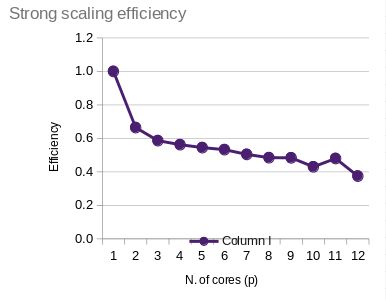
\includegraphics[scale=0.5]{images/mpi_strong.png}
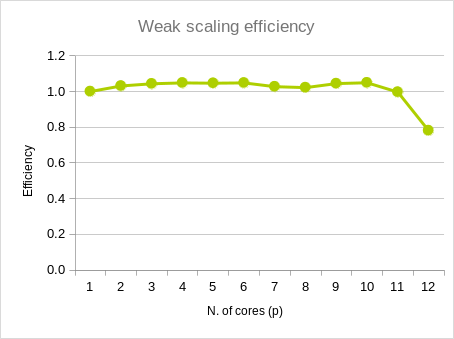
\includegraphics[scale=0.5]{images/mpi_weak.png}
\begin{table}[!ht]
    \centering
    \begin{tabular}{|l|l|l|l|l|l|l|}
    \hline
        p & t1 & t2 & t3 & t4 & t5 & ~ \\ \hline
        1 & 0.003678 & 0.003035 & 0.002918 & 0.003182 & 0.003141 & ~ \\ \hline
        2 & 0.006129 & 0.006134 & 0.006129 & 0.006159 & 0.006041 & ~ \\ \hline
        3 & 0.009250 & 0.010712 & 0.009162 & 0.009259 & 0.008583 & ~ \\ \hline
        4 & 0.012803 & 0.011717 & 0.011680 & 0.012336 & 0.013111 & ~ \\ \hline
        5 & 0.014638 & 0.014620 & 0.015177 & 0.015184 & 0.013320 & ~ \\ \hline
        6 & 0.017274 & 0.015946 & 0.017011 & 0.016703 & 0.017459 & ~ \\ \hline
        7 & 0.019960 & 0.020302 & 0.020186 & 0.018834 & 0.019676 & ~ \\ \hline
        8 & 0.021634 & 0.029037 & 0.021791 & 0.022178 & 0.022520 & ~ \\ \hline
        9 & 0.024613 & 0.023907 & 0.025140 & 0.024692 & 0.024487 & ~ \\ \hline
        10 & 0.027618 & 0.027551 & 0.027602 & 0.027214 & 0.026683 & ~ \\ \hline
        11 & 0.028849 & 0.029816 & 0.029343 & 0.029504 & 0.029187 & ~ \\ \hline
        12 & 0.032244 & 0.031859 & 0.032763 & 0.032379 & 0.033032 & ~ \\ \hline
    \end{tabular}
\end{table}
\newline
La ragione per cui lo speedup diminuisce nella dodicesima iterazione è che il thread probabilmente viene usato dal sistema operativo.
\section*{Conclusioni}
Ho ottenuto uno speedup significativo sia nella versione MPI che nella versione OpenMP.
La differenza principale tra il programma MPI e il programma OpenMP è la mancanza di dynamic scheduling nella versione MPI.
Questo si traduce in performance peggiori nella versione MPI, dato che il workload è sbilanciato.
Per ottimizzare meglio il programma, si potrebbe cercare di rimuovere la loop-carried dependency, o cercare di implementare il dynamic scheduling di OpenMP in MPI.
Un'altra possibile ottimizzazione è aumentare la cache locality iterando sui displacement x e y separatamente.
Questo consente al programma di dover tenere nella cache solo il displacement corrente, effettivamente raddoppiando il numero di displacement nella cache.
Ho inoltre notato che il numero di intersezioni non sono esattamente uguali tra versione parallellizzata e seriale, ma differiscono di circa lo 0.5\% alla ventesima iterazione.
Dopo una sessione di debugging, credo che questo sia dovuto al fatto che i float che rappresentano i displacement vengono sommati in un ordine diverso, dando origine così a risultati leggermente inconsistenti.
\printbibliography
\appendix

\end{document}